\documentclass{article}

\usepackage{amsmath}
\usepackage{amssymb}
\usepackage{tikz}
\usepackage{tikzit}

\usepackage{authblk}
\usepackage{blindtext}

\usepackage{url}
\usepackage{cite}
%% -------------------------------------- Declare the layers
\pgfdeclarelayer{nodelayer}
\pgfdeclarelayer{edgelayer}
\pgfsetlayers{edgelayer,nodelayer,main}
% Node styles
\tikzstyle{black circle}=[fill=white, draw=black, shape=circle, tikzit shape=circle]
\tikzstyle{Arrow}=[->]

% Edge styles
\tikzstyle{new edge style 0}=[->]

\title{Large-scale mapping of antigenic relationships in Sars-CoV-2}
\author[1,4]{Peter C. Jentsch}  
\author[3,5]{Finlay Maguire}
\author[1,2]{Samira Mubareka}
\affil[1]{Sunnybrook Research Institute, Toronto, Canada}
\affil[2]{University of Toronto, Toronto, Canada}
\affil[3]{Dalhousie University, Halifax, Canada}
\affil[4]{Simon Fraser University, Burnaby, Canada}
\affil[5]{Shared Hospital Laboratory, Toronto, Canada}
\date{\today}                    
\setcounter{Maxaffil}{0}
\renewcommand\Affilfont{\itshape\small}

\begin{document}

\maketitle

\section{Background}

The rapid and widespread adoption of immunization has saved millions of lives in the COVID-19 pandemic.
As the world's population gains immune experience with Sars-CoV-2, either through previous infection or vaccination, antigenic drift has given rise to new variants that exhibit significant immune escape\cite{yewdellAntigenicDriftUnderstanding2021}.
Similar to the annual reformulation of influenza vaccinations, public health planning has shifted resources towards increasing resilience against the emergence of SARS-CoV-2 variants.
The Moderna and Pfizer mRNA vaccine boosters were updated accordingly to a bivalent version, including both the ancestral spike protein and the spike protein from the BA.1 lineage of the Omicron variant, the first variant to exhibit major immune escape.
In the mean time, the BA.4 and BA.5 Omicron sublineages have become widespread, becoming the majority of COVID-19 cases by July 2022 \cite{wilhelm2022early}.

Since these sublineages are also antigenically distinct from their BA.1 ancestors \cite{cao2022ba}, development of bivalent mRNA boosters which cover BA.4 and BA.5 quickly followed \cite{chalkias2022bivalent}.
The uptake of updated vaccine boosters will undoubtedly reduce the burden of new variants on health systems worldwide, but perhaps we can do better than a reactive approach.
The level of genomic surveillance during this pandemic has been unprecedented, and many new methods have been developed to take advantage of the quantity of data collected.
Understanding this immune landscape and the dynamics of viral evolution within it will be key to remaining in control of the resulting antigenic arms race.

Mapping antigenic relationships between related pathogens was pioneered with Influenza A \cite{lapedesGeometryShapeSpace2001}. 
The immune response of an antiserum to a different antigen, antigenic distance, can be quantified as a reduction in concentration of the newly introduced antigen.
These relationships can be measured between many related strains of a pathogen, to create a map of changing immune responses through the evolution of the pathogen.
With manifold reduction techniques such as multidimensional scaling, these relationshps can often be approximately represented in two or three dimensional cartesian maps, explicitly showing the antigenic drift of the pathogen.
This technique was used to map the antigenic evolution of Influenza A, and argue that it can be understood as primarily occurring in only two dimensions \cite{lapedesGeometryShapeSpace2001, smithMappingAntigenicGenetic2004}.
Wilks et al. have developed upon this technique to create an antigenic map of approximately 17 major variants of Sars-CoV-2 from serum neutralization assays, and further argue that a two-dimensional map is an adequate approximation of the landscape \cite{millerAntigenicSpaceFramework2021, wilksMappingSARSCoV2Antigenic2022, van2022mapping}. 

This work on data-driven approximations of antigenic space motivates the development of models that explicitly incorporates data on antigenic relationships obtained from these neutralization assays.
The dynamics of related pathogen strains evolving within a shared host population can rapidly become intractable, and therefore researchers have devised models which can manage this complexity.
One method is to constrain the possible viral strains to points on a finite one or two dimensional lattice, thereby making the analysis of strain evolution tractable \cite{gogDynamicsSelectionManystrain2002} . 
In two dimensional strain space, cross-immunity of a pathogen is given specified by an arbitrary function of the euclidean distance between strains, and mutation is implemented as discrete diffusion with some fixed speed. 
To accurately parameterize these models, the map of antigenic space should use as much genomic information as is available.
Fortunately, for Sars-CoV-2, the most sequenced biological entity, we have a huge amount of information. 
With millions of the samples in the global SCV2 tree, our combined knowledge of the antigenic space of SCV2 could be orders of magnitude more detailed.
In this manuscript, we describe methods for constructing more detailed antigenic maps using a subset this genomic diversity, and provide some examples of these maps.

% Previous work on these models do not use data to estimate parameters, focusing on broad characterization of dynamics with numerical or analytical approaches. However, genomic data does include a huge amount of admittedly very noisy information. 
% There is some recent work on parameter estimation by comparing simulated phylogeny with observed phylogeny using a suite of summary statistics for tree structures \cite{danesh2021quantifying,leventhal2012inferring,saulnier2017inferring}, but these models do not explicitly include genomic structure, which might provide additional inferential power. 

\section{Methods}

To add viral genomes to our map without obtaining explicit antigenic distances via laboratory assays, we need some method of estimating antigenic distances from genomic data. 
There are two additional sources of information that we use for this interpolation.
Deep mutational scanning of the receptor binding domain (RBD) of the Sars-CoV-2 genome has been used to measure the polyclonal antibody binding affinity for a mutation at every nucleotide in the RBD \cite{starr2020deep}.
Using this data, it is possible to approximate the polyclonal binding affinity for an arbitrary given RBD sequence \cite{greaney2022antibody}.
This algorithm is gives the binding affinity for a given RBD is returned by the aformentioned tool as a fraction between zero and one, where a binding affinity of one represents perfect binding and zero represents no binding, or complete antibody escape.
While antigenic distance is more complex than just antibody binding affinity to the viral RBD, we include it as one aspect of our antigenic distance approximation. 

The second metric we use is the number of SNPs between two genomes, because identical viral genomes should receive very similar immune reactions, and genomes that have many mutations between them will likely have provoke different immune reactions.
However, the degree to which a given SNP will affect the antigenic escape of the mutated virus depends significantly on the location and base of the SNP in the genome. 
For instance, since the spike protein is the main antigen of the virus, mutations in the spike protein are far more relevant than mutations in other proteins \cite{harvey2021sars}.
To that end, we weight SNPs by the frequency with which they independently reoccur within in the global tree \cite{attwood2022phylogenetic}.
This is done by counting the  sites from the global SCV2 tree created with USHER \cite{turakhia2021ultrafast}, using the software tool matUtils \cite{mcbroome2021matutils}.



For each pair of genomes $g_i$ and $g_j$ ($i\neq j$) aligned with the reference, first we find the closest lineages in the existing antigenic map to $g_i$, and $g_j$ using the Pango lineage assignments of $g_i$ and $g_j$. Precisely, given the set of lineages examined by \cite{wilksMappingSARSCoV2Antigenic2022}, we first approximate the position of new genomes by mapping them to the most recent ancestor lineage present in the map using their Pango lineage assignment, computed with the Pangolin software tool \cite{o2021assignment}. Using these closest mapped lineages, we use their mapped coordinates $x_i$ and $x_j$ as a first approximation for the antigenic distances.
Assume the polyclonal binding affinity is given by $B(g)$ (computed by \cite{greaney2022antibody}), where $g$ is some viral genome sequence. Further let $g_i^{(k)}$ be the $k$th nucleotide base in $g_i$ and $\chi(g_i^{(k)},g_j^{(k)})$ the two argument indicator function given by equation \ref{indicator}.
\begin{equation}
        \chi(a,b) =   \begin{cases}
        1 & \text{if $a = b$} \\
        0 & \text{otherwise} \\
    \end{cases}
    \label{indicator}
\end{equation}
Assume $h^{(k)}$ is a vector containing the number of homoplasic mutations at site $k$ in the global tree, and $W>0$ is a real number denoting the weighting of the extra distances.
Then we compute the distance between $g_i$ and $g_j$ as given by equation \ref{distanceeqn}.
\begin{equation}
    d(g_i,g_j) = \lVert x_i - x_j \rVert + W \frac{B(g_i) + B(g_j)}{2}\frac{\sum_k \chi\left(g_i^{(k)},g_j^{(k)}\right) h^{(k)}}{\sum_k h^{(k)}}
    \label{distanceeqn}
\end{equation}
Computing $d(g_i, g_j)$ for every pair of Sars-CoV-2 genomes $g_i$ and $g_j$ gives a distance matrix between all genomes in the sample.
We use multidimensional scaling (MDS) as in \cite{wilksMappingSARSCoV2Antigenic2022, lapedesGeometryShapeSpace2001} to place the genomes in 2 dimensional euclidean space in a way that closely approximates their distances with respect to $d$.


The dataset we use for this is the set of public genomes made available by the NCBI (CITE). 
To avoid sampling bias we take only the genomes sequenced as a result of random sampling, for a total of 1,895,794 unique Sars-CoV-2 genomes.
However, we only consider the SNPs in the RBD, plus the top 100 most frequent SNPs with respect to $h$, because the weight assigned to other SNPs is largely negligible. 
This simplification reduces the total number of unique genomes to 18533, which is much more tractable for processing with commonly available MDS software packages.


\section{Results}


\begin{figure}
    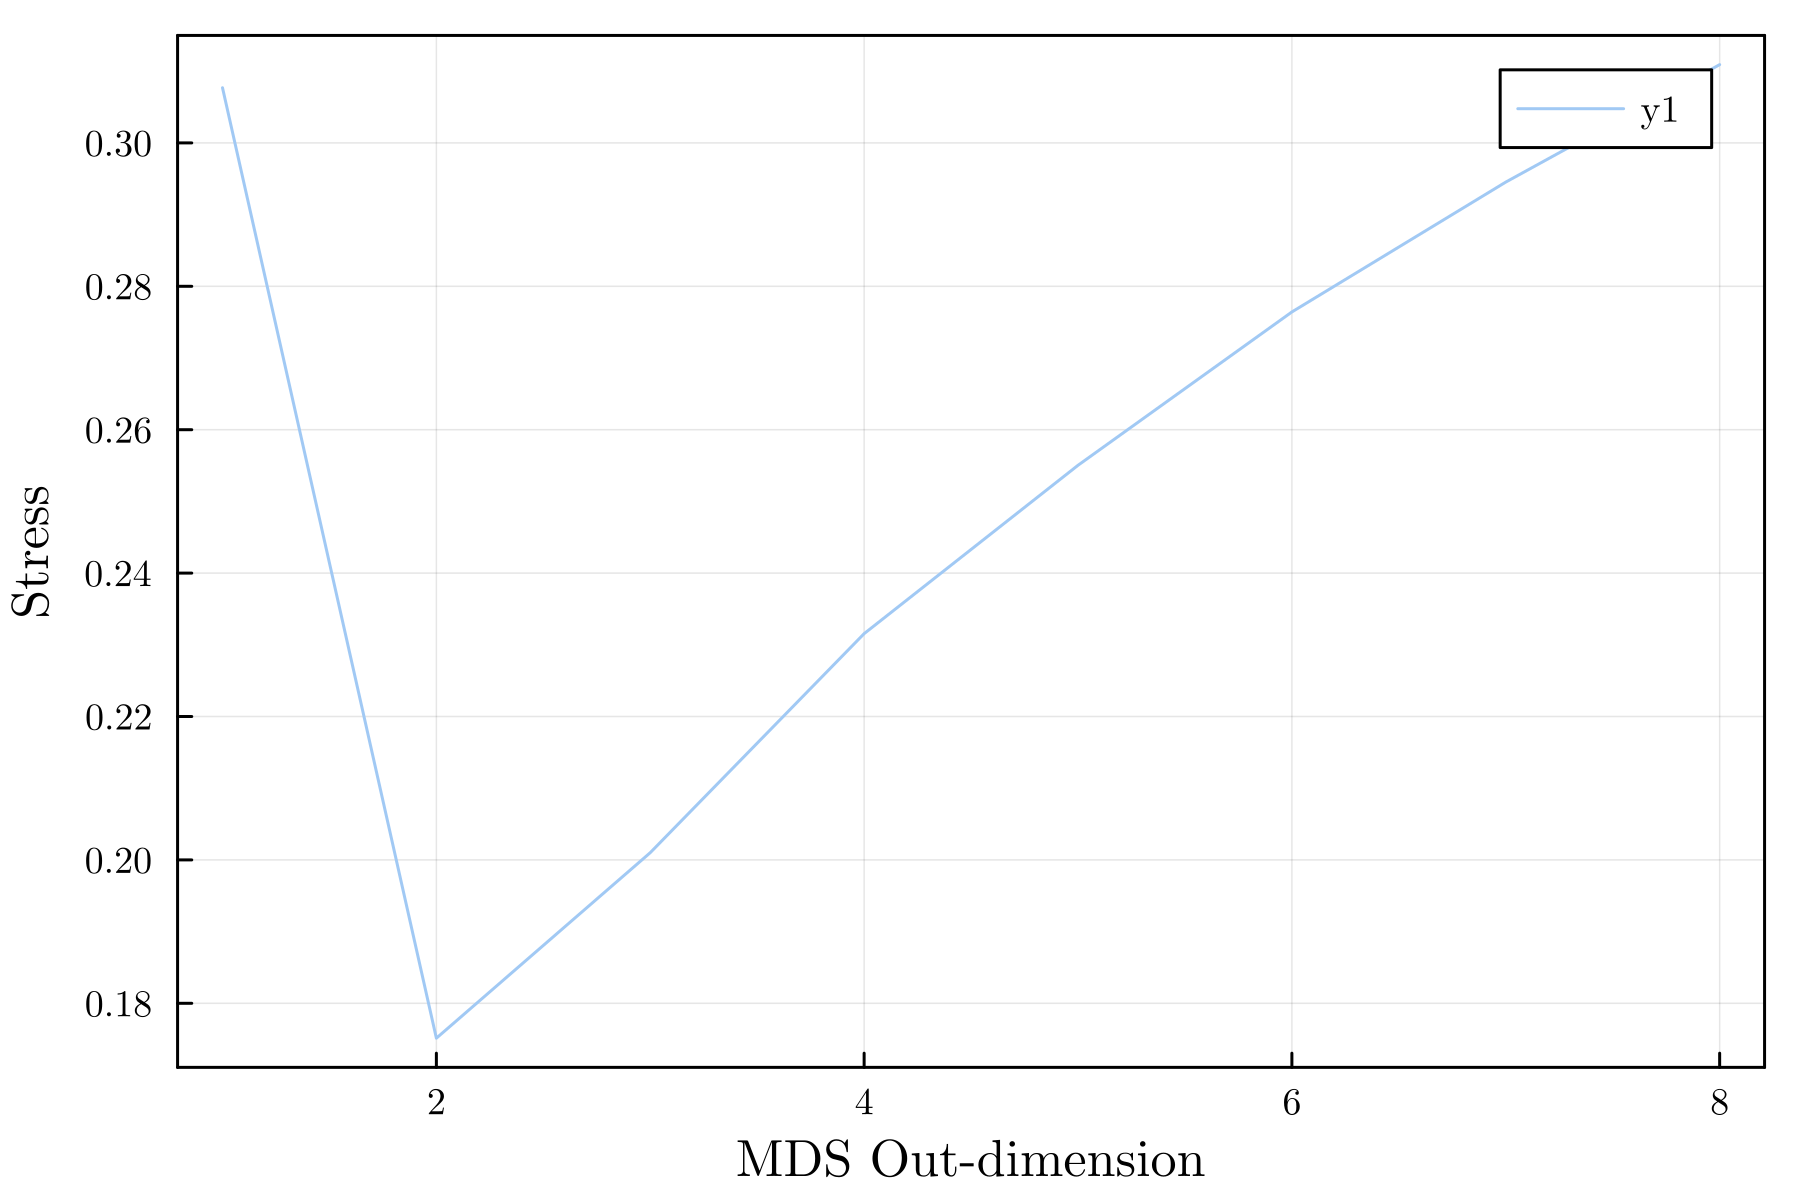
\includegraphics[width=\textwidth]{../SarsEvoModel/plots/combined_mds_stress.png}    
    \caption{An output dimension of 2 minimizes the stress in the multidimensional scaling dimension reduction.}
\end{figure}%likely because the wilks points are in a 2d plane..

\begin{figure}
    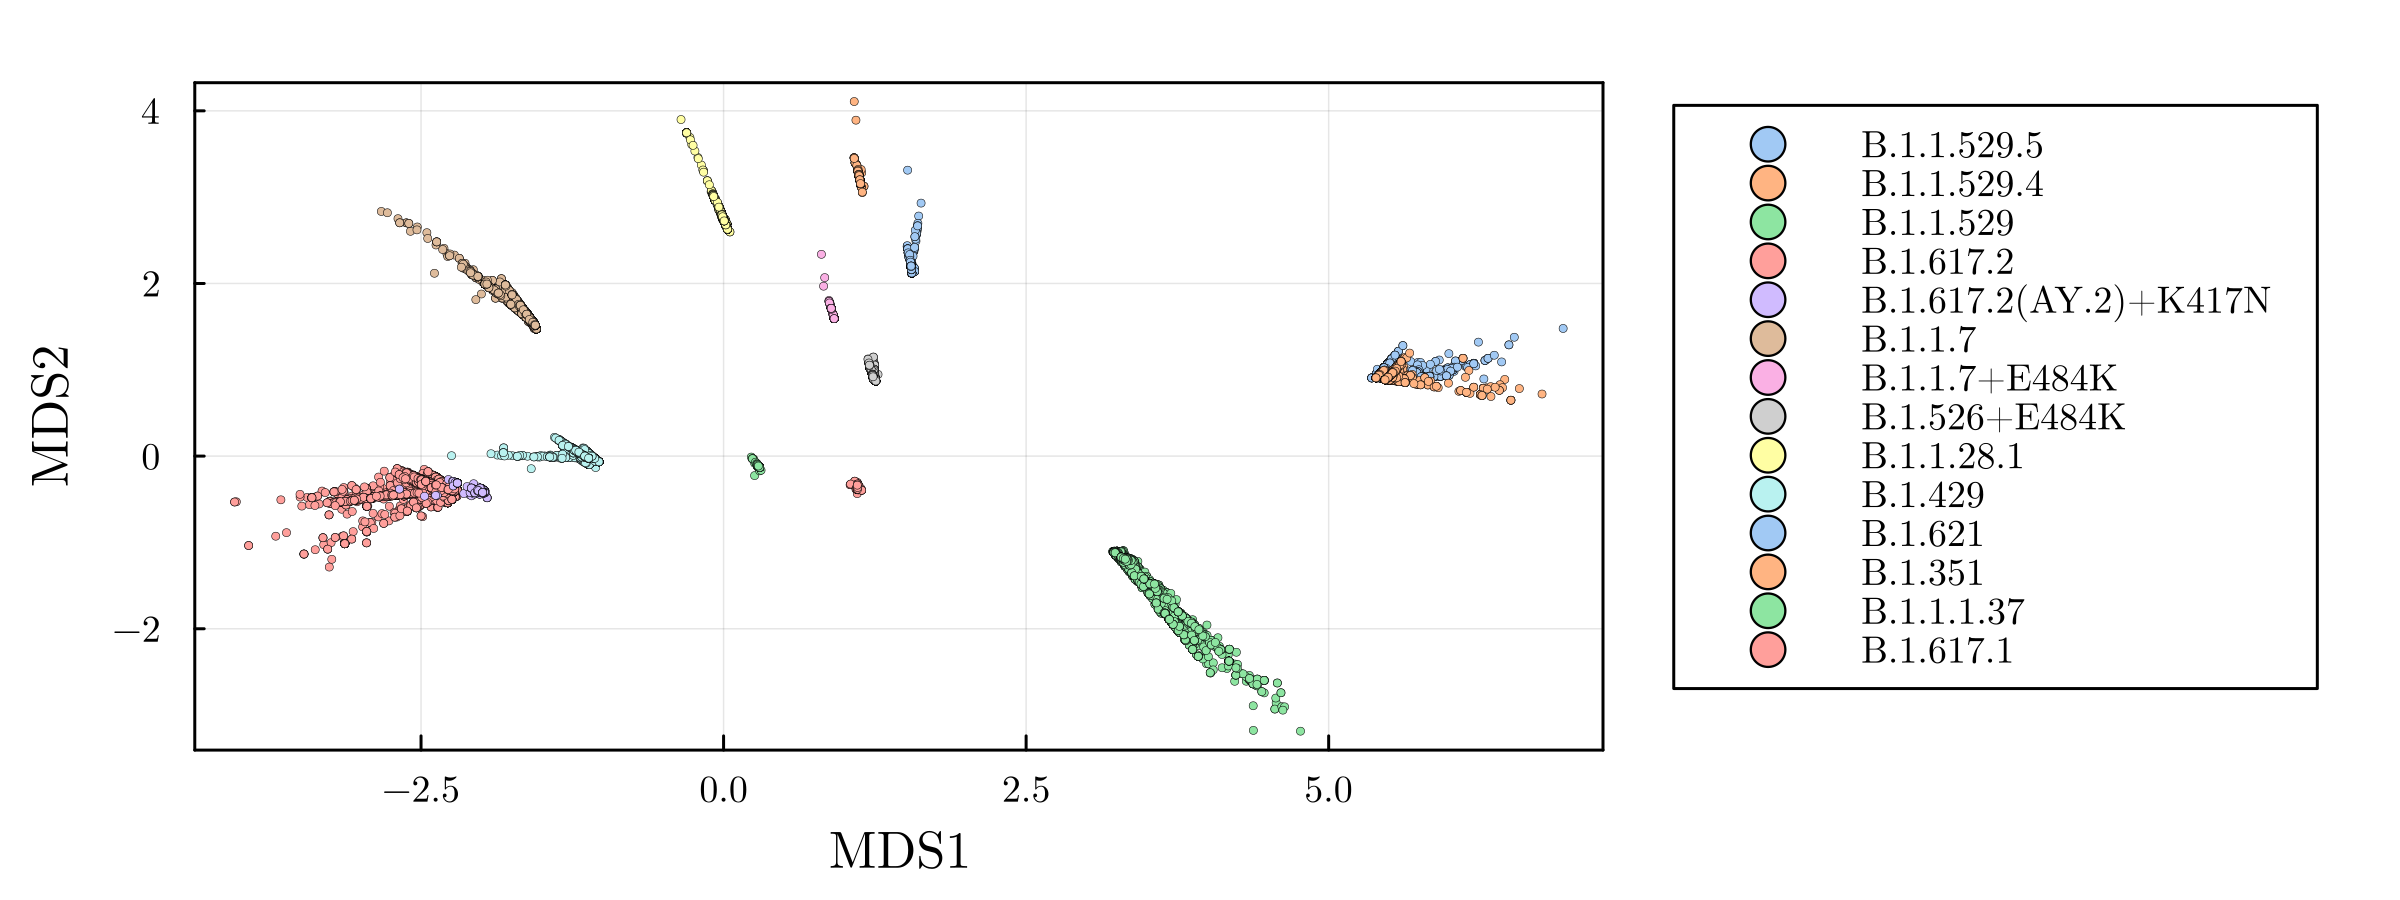
\includegraphics[width=\textwidth]{../SarsEvoModel/plots/homoplasy_usa/homoplasy_usa_mds_multidimensional_scaling.png}    
    \caption{Map of the } 
\end{figure}



% \section{Model}



% \begin{equation},,
%     S_{ij}'(t) = -\sum_{kl} \beta_{kl} \sigma_{ijkl} S_{ij} I_{kl} + \gamma R_{ij}  \label{Seqn}
% \end{equation}
% \begin{equation}
%     I_{ij}'(t) = \beta_{ij} S_{ij} I_{ij} - \xi I_{ij} + M \left(- 4I_{ij} + I_{i-1,j}  + I_{i+1,j} + I_{i,j-1} + I_{i,j+1} \right) \label{Ieqn}    
% \end{equation}
% \begin{equation}
%     R_{ij}'(t) = \xi I_{ij} - \gamma R_{ij}  \label{Reqn}
% \end{equation}


% \begin{table}[h!]
%     \begin{center}
%         \begin{tabular}{c|p{8cm}}
%             Symbol & Description \\
%             \hline
%             \hline
%             $N$ & Size of variant grid \\
%             $S_{ij}$ & Population susceptible to variant $(i,j) \in [0,N]^2$ \\
%             $I_{ij}$ & Population infected by variant $(i,j) \in [0,N]^2$\\
%             $R_{ij}$ & Recovered/Immune to variant $(i,j) \in [0,N]^2$\\
%             $\sigma_{ijkl}$ & Probability that exposure to variant $(i,j)$ causes immunity \newline to variant $(k,l)$\\
%             $\beta_{ij}$ & Transmission rate of variant $(i,j)$\\
%             $\xi$ & Recovery rate of all strains \\
%             $\gamma$ & Rate of immunity loss of all strains \\
%     \end{tabular}
%     \caption{Table of symbols for Model 2}

%     \label{variables_2}
%     \end{center}
% \end{table}

    

% Equations \ref{Seqn}-\ref{Reqn} represent the model of \cite{gogDynamicsSelectionManystrain2002} with a two-dimensional strain space, with a few changes to better reflect mechanisms of of Sars-CoV-2. I have added an immunity period, changing the model to an SIRS mechanism, and removed the vital dynamics, as I do not think natural population birth rates are significant in the time scale of the pandemic. A key assumption made by this model is that exposure grants complete immunity to some fraction of individuals, rather than partial immunity (interpreted as reduced transmission rates) to all exposed individuals. Many other methods of dealing with cross-immunity are possible, but this method gives a simpler state space \cite{Castillo_Chavez_Blower_Driessche_Kirschner_Yakubu_2002}.


% To incorporate vaccination, consider each vaccine affecting a different region of strain space. That is, for a vaccine $v$ we can associate a matrix $v_{ij} \in [0,1]$ which determines the relative effect of that vaccine on the immunity of hosts to strain $i,j$. The function $eta(t)$ represents some base rate of vaccination. This results in the following equations for $S_{ij}'(t)$ and $ R_{ij}'(t) $ (the infected equation \ref{Ieqn} is unchanged).


% \begin{equation}
%     S_{ij}'(t) = -\sum_{kl} \beta_{kl} \sigma_{ijkl} S_{ij} I_{kl} + \gamma R_{ij} -  \eta(t) v_{ij} S_{ij} \label{Seqn}
% \end{equation}
% \begin{equation}
%     R_{ij}'(t) = \xi I_{ij} - \gamma R_{ij} + \eta(t) v_{ij} S_{ij} \label{Reqn}
% \end{equation}


% This model could be used to test the effect of NPIs on Sars-CoV-2 evolution. Mechanisms for NPIs and additional compartments for heterogeneity are straightforward to add to the model equations. If a given NPI mechanism is more able to fit data with a mechanism that does not act on all strains equally, then this could be evidence that NPIs are affecting Sars-CoV-2 evolution. 

% \subsection{Continuous strain-space}

% The above model can be viewed as simply a first-order finite difference approximation of a continuous space reaction-diffusion model. Accordingly, we can generalize it to continuous strain-space as
 
% \begin{equation}
%     S_t(x,y,t) = \int_{-\infty}^{\infty} \int_{-\infty}^{\infty} \beta(x',y') \sigma(x,y,x', y') S(x,y,t) I(x',y',t) dx' dy' + \gamma R_{ij} -  \eta(t) v(x,y) S(x,y,t)\label{Seqn_cts}
% \end{equation}
% \begin{equation}
%     I_t(x,y,t) = \beta(x,y) S(x,y,t) I(x,y,t)- \xi I(x,y,t) + M \left(I_x(x,y,t)  + I_y(x,y,t)  \right) \label{Ieqn_cts}    
% \end{equation}
% \begin{equation}
%     R_t(x,y,t) = \xi I(x,y,t)I(x,y,t) - \gamma R(x,y,t) + \eta(t) v(x,y) S(x,y,t) \label{Reqn_cts}
% \end{equation}

% where $\beta, \sigma, v$ have been generalized to their continuous counterparts. This formulation is similar to the 1-dimension strain space model described in \cite{Bessonov_Bocharov_Meyerhans_Popov_Volpert_2021}. Then, given a dispersion kernel $K(x,y) \in L_2: \mathbb{R}^2 \to \mathbb{R}$ this can be generalised to non-local diffusion as follows

% \begin{equation}
%     I_t(x,y,t) = \beta(x,y) S(x,y,t) I(x,y,t)- \xi I(x,y,t) + M \left(\int_{-\infty}^{\infty} \int_{-\infty}^{\infty} K(x-x',y-y')I(x',y',t) dx' dy' \right) \label{Ieqn_cts_nonlocal}    
% \end{equation}



% \section{Methods}
% To interpolate more genomic data into this map, we begin with 


% Citation for homoplasy stuff?
% z

\bibliographystyle{plain}
\bibliography{ref.bib}

\end{document}  


% \section{Model}
% \label{model}
% \begin{itemize}
%     \item The structure of the model is Susceptible-Exposed-Infected-Asymptomatic-Recovered, outlined in Figure \ref{model_structure}.
%     \item The mRNA vaccine lowers transmission rates and increases the proportion of asymptomatic infections compared to the AstraZeneca vaccine
%     \item Focus on infections in two lineages
%     \item Each lineage has different infection rates, recovery times, and latent periods
%     \item Co-infection negligible 
%     \item Time scale short enough that recovery from either infection grants immunity
%     \item Strains interact in the model only in that they compete for hosts
%     \item Vaccination immunity does not wane over model timescale (i.e., single pandemic wave)
%     \item Vaccination reduces infection rate by a proportion
%     \item Some constant fraction of cases are asymptomatic
%     \item Vaccination rate is constant (not necessary since we have data on exact vaccination rates)
%     \item Transmission rate is affected by current level of state policy (determined by the stringency index) and the current level of infection (corresponding to social distancing)
% \end{itemize}

% \begin{figure}[h!]
%     \centering
%     \begin{tikzpicture}
	\begin{pgfonlayer}{nodelayer}
		\node [style=black circle] (0) at (0, 0) {};
		\node [style=black circle] (1) at (-1, 0) {};
		\node [style=black circle] (2) at (1, 0) {};
		\node [style=black circle] (3) at (2, 0) {};
		\node [style=black circle] (4) at (-2, 0) {};
		\node [style=rectangle] (5) at (-2, 1) {$V_i$};
		\node [style=rectangle] (6) at (-2, 4) {$S_i$};
		\node [style=rectangle] (7) at (-2, 2) {$R_i$};
		\node [style=rectangle] (8) at (-2, 3) {I_i};
	\end{pgfonlayer}
\end{tikzpicture}
v   
% \caption{State diagram of model with two different types of vaccination and strong competition. Variables are described in Table \ref{variables}}
% \label{model_structure}
% \end{figure}

% \subsection*{Further extensions}

% \begin{itemize}
%     \item Compartments will be added to test the effect of population and policy heterogeneity on viral prevalence
%     \item Postal code data for genomes would enable us to track mutations in space, and compare to small variations PHU-level closure data in a network model such as \cite{Fair_Karatayev_Anand_Bauch_2021}
    
%     \item There is a lot of genomic information not captured in high-level lineage assignments that could be used in a more 
%     detailed 
%     more of 
%     viral strain competition

%     \item Another technique that is popular for estimating epidemiological parameters, particularly in the comparison of VoC is a semi-mechanistic approach (e.g.\cite{Cauchemez_Nouvellet,Fraser_2007,Mishra_Berah_Mellan_Unwin_Vollmer_Parag_Gandy_Flaxman_Bhatt_2020,Nouvellet_Cori, Wallinga_Lipsitch_2007, Brown_Joh_Buchan_Daneman_Mishra_Patel_Day_2021})
% \end{itemize}


% \begin{table}[h!]
%     \begin{center}
%     \begin{tabular}{c|l}
%             Symbol & Description \\
%             \hline
%             \hline
%             $S$ & Susceptible, unvaccinated \\
%             $A^{(i)}$ & Asymptomatically infected with $i$th variant\\
%             $I^{(i)}$ & Infected with $i$th variant \\
%             $E^{(i)}$ & Exposed to $i$th variant \\
%             $R^{(i)}$ & Recovered from $i$th variant \\
%             $S_{V_i}$ & Susceptible, unvaccinated \\
%             $A^{(i)}_{V_i}$ & Asymptomatically infected with $i$th variant, vaccinated by $i$th vaccine\\
%             $I^{(i)}_{V_i}$ & Infected with $i$th variant, vaccinated by $i$th vaccine\\
%             $E^{(i)}_{V_i}$ & Exposed to $i$th variant, vaccinated by $i$th vaccine\\
%             $R^{(i)}_{V_i}$ & Recovered from $i$th variant, vaccinated by $i$th vaccine\\
%             $C(t, \Sigma_i I^{(i)}) $ & Function reducing transmission rate due to NPIs \\
%             $\beta_i$ & Transmission rate of $i$th variant \\
%             $\eta_i(t)$ & Vaccination rate for $i$ vaccine\\
%             $s$ & Fraction of asymptomatic \\
%             $\sigma^{(i)}$ & Inverse of latent period for $i$th variant \\
%             $\gamma^{(i)}$ & Recovery rate for $i$th variant \\
%             $\nu_{V_i}$ & Infectiousness reduction for vaccination by $i$th vaccine \\
%     \end{tabular}
%     \caption{Table of symbols for Model 1}

%     \label{variables}
%     \end{center}
% \end{table}